\documentclass[11pt,a4paper]{article}
\usepackage[margin=25mm]{geometry}
\usepackage[T1]{fontenc}
\usepackage{lmodern}
\usepackage{graphicx}
\usepackage{booktabs}
\usepackage{tabularx}
\usepackage{amsmath}
\usepackage{xcolor}
\usepackage[colorlinks=true,linkcolor=blue!60!black,urlcolor=blue!60!black]{hyperref}
\usepackage{caption}
\captionsetup{font=small,labelfont=bf}
\usepackage{microtype}
\usepackage{needspace}

\setlength{\parskip}{4pt}
\setlength{\parindent}{0pt}

\newcommand{\finding}[1]{\medskip\noindent\textbf{#1}\par\smallskip}

\begin{document}

\tableofcontents
\newpage

\section{Executive summary}

NeuroFoil is an end-to-end aerodynamic data engine: it plans and executes an
automated Reynolds-Averaged Navier--Stokes (RANS) campaign, curates the result
into a provenance-controlled dataset, trains surrogate models for scalar force
coefficients and full surface-pressure distributions, and serves predictions
with split-conformal uncertainty intervals and out-of-domain detection. This
report documents the completed system using only measured artifacts from the
repository.

The campaign attempted the full 504-case design (21 NACA four-digit airfoils
$\times$ 4 Reynolds numbers $\times$ 6 angles of attack, medium C-grid,
$k$--$\omega$ SST, incompressible). Coverage is \textbf{400/504}: 374 cases
converged cleanly under strict criteria; 26 solved but failed the convergence
window; 104 operating points were excluded after the physical cause of their
failure---steady-RANS limit cycles at negative incidence and thin-airfoil
stall---was verified from force histories across three independent campaign
attempts. All 21 airfoils retain converged data at all four Reynolds numbers.

A surrogate trained on the 375 converged rows (including one adjacent
validation point) was evaluated on grouped per-airfoil holdouts---airfoils
never seen in training. Extrapolation $R^2$ is 0.966 for $C_L$, 0.933 for
$C_D$ and 0.860 for $C_m$; the surface-pressure decoder reaches $R^2 = 0.892$
on unseen geometries, and integrating its predicted pressure jump reproduces
the predicted lift with $R^2 = 0.983$ (physics consistency). Empirical
split-conformal coverage on the unseen-airfoil test set is 0.951 ($C_L$),
0.918 ($C_D$), 0.967 ($C_m$) and 0.957 ($C_p$) against the 0.95 nominal level.
At inference, queries far from the training manifold are flagged by a
Mahalanobis domain guard rather than answered with false confidence.

The dataset, trained bundle, quality-control tooling, mesh-sensitivity study,
and every number in this report are reproducible from the repository.

\section{System architecture}

\begin{figure}[htbp]
\centering
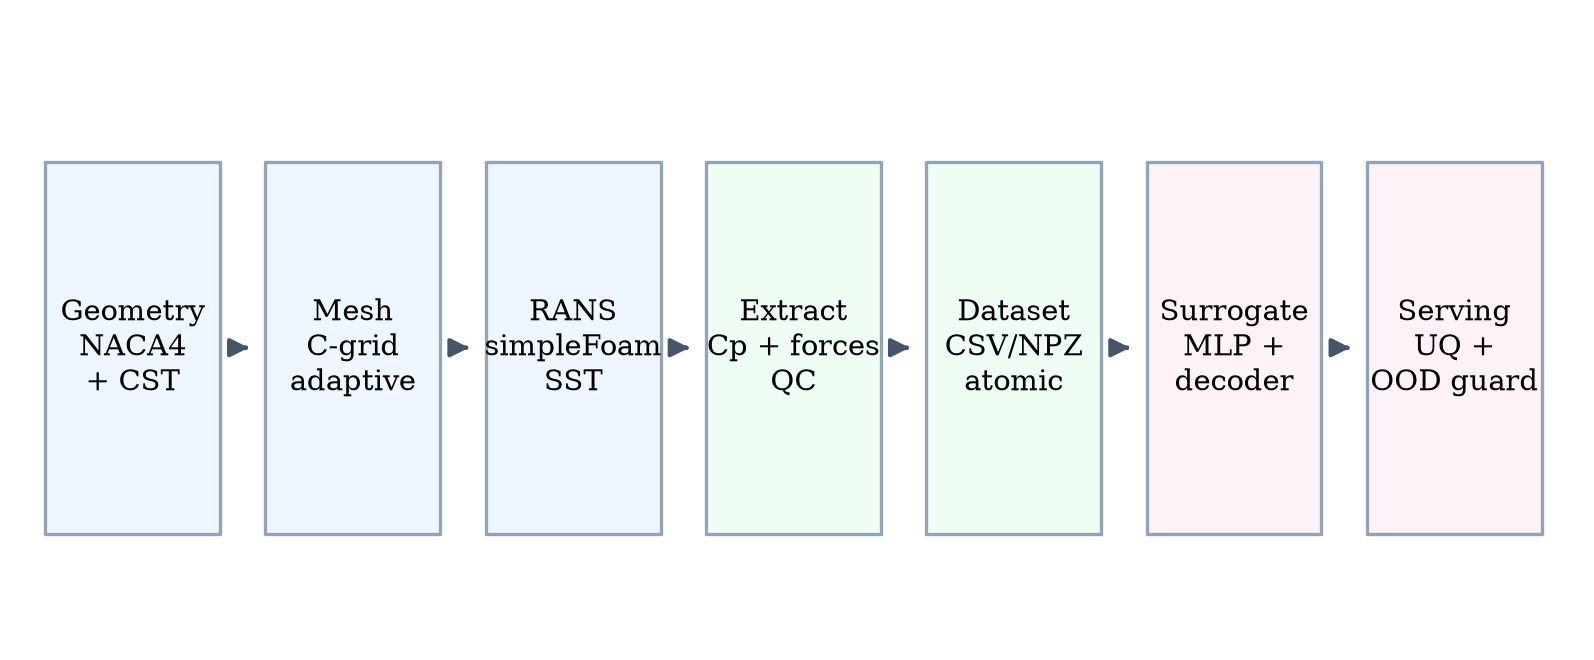
\includegraphics[width=0.98\textwidth]{figures/fig_architecture.png}
\caption{NeuroFoil pipeline. Each stage is a repository module; the dataset
stage persists atomically after every completed case.}
\label{fig:arch}
\end{figure}

The pipeline has seven stages (Figure~\ref{fig:arch}). Geometry generation
emits NACA four-digit shapes with closed trailing edges and their
fifth-order CST fits; the mesher writes a six-block structured C-grid;
\texttt{simpleFoam} solves incompressible $k$--$\omega$ SST RANS; the
extractor resamples surface pressure onto a common 161-point chord grid and
evaluates convergence from force histories; the dataset layer stores every
completed case atomically (temporary-file rename) into a CSV/NPZ pair with
per-row provenance; the training notebook produces a bundle of NumPy weights,
scalers and conformal quantiles; and the inference engine loads that bundle
with domain-applicability guards.

\section{CFD campaign methodology}

\subsection{Design of experiments}

The grid is 21 airfoils $\times$ 4 Reynolds numbers
($10^6$, $2\times10^6$, $3\times10^6$, $6\times10^6$) $\times$ 6 angles of
attack ($-6^\circ$, $-2^\circ$, $+2^\circ$, $+6^\circ$, $+10^\circ$,
$+14^\circ$) = 504 cases. Three literature anchors (NACA 0012, 2412, 4412)
lead the list; the remaining 18 shapes are drawn by Latin hypercube sampling
over camber, camber position and thickness with a fixed seed (42), giving a
deterministic, reproducible shape set. Farfield radius and wake length are 15
chords; the first cell height is $4\times10^{-6}$ chords, targeting
$y^+ \approx 1$ at $Re = 6\times10^6$.

\subsection{Mesh generation and the adaptive split fallback}

The C-grid is split at $x/c = 0.30$ into nose and aft blocks. Five sampled
geometries (NACA 1207, 3208, 3210, 6313, 6211) produced meshes whose maximum
non-orthogonality exceeded the 70-degree acceptance limit at the default
split---by margins from 0.16 to 13.9 degrees. A mesh-only parameter study
(no solver runs) showed the maximum non-orthogonality decreases monotonically
as the split moves forward; a uniform fallback split at $x/c = 0.08$ brings
all five shapes under the limit (47.98--64.17 degrees) while preserving cell
count (18{,}048), first-cell height, farfield and mesh level. The pipeline now
applies this fallback automatically when the default mesh is rejected, and
records the split actually used in each dataset row. The fallback recovered
all 120 cases of the five affected geometries.

\subsection{Solver configuration and convergence adjudication}

Each case runs \texttt{simpleFoam} with potentialFoam initialisation,
under-relaxation (pressure 0.1, velocity 0.3, $k$/$\omega$ 0.5), second-order
limited-linear convection, and a 6000-iteration budget (3000 in the first
campaign pass; cases do not stop early, so the budget is a hard iteration
cap). A case is labelled \emph{converged} only if the standard deviations of
$C_L$, $C_D$ and $C_m$ over the final 100 iterations fall below
$5\times10^{-4}$, $2\times10^{-4}$ and $5\times10^{-4}$ respectively;
\emph{unconverged} cases that still produce finite, extracted fields are
retained with their data but excluded from training.

\subsection{Persistence and checkpointing}

Every completed case is committed to the CSV/NPZ pair atomically before the
next case starts, with rollback logic if either write fails. Interruptions
(costly thermal shutdowns among them) are therefore free: a restarted
campaign prints its resume count and continues. Failed attempts are recorded
with \texttt{success=False} and retried automatically; the last attempt per
case identifier is authoritative.

\section{Verification and validation}

\subsection{Solver checks}

Two NACA 0012 pipeline checks anchor the campaign to known behaviour
(incompressible $k$--$\omega$ SST, medium mesh, 3000 iterations):

\begin{table}[htbp]
\centering
\caption{NACA 0012 solver checks (medium mesh).}
\label{tab:solverchecks}
\begin{tabular}{lrrrl}
\toprule
Case & $C_L$ & $C_D$ & $C_m$ ($c/4$) & Status \\
\midrule
$\alpha = 0^\circ$, $Re = 6\times10^6$ & $-0.0042$ & $0.00879$ & $+0.0008$ & converged \\
$\alpha = 4^\circ$, $Re = 6\times10^6$ & $+0.4388$ & $0.00951$ & $+0.0024$ & converged \\
\bottomrule
\end{tabular}
\end{table}

The near-zero symmetric result and the converged $\alpha = 4^\circ$ case give
an implied two-point lift slope of $6.29\ \mathrm{rad}^{-1}$, close to
thin-airfoil theory ($2\pi \approx 6.28$). The fully turbulent drag level
($C_D \approx 0.0095$) sits above the cited transitional experimental value
($\approx 0.0081$), as expected without a transition model.

\subsection{Grid sensitivity}

A five-run study on NACA 0012 at $\alpha = 4^\circ$, $Re = 6\times10^6$
compared coarse (9{,}000 cells), medium (18{,}048) and fine (36{,}000) meshes
at equal convergence depth (Figure~\ref{fig:mesh}). At 6000 iterations the
three levels agree within 0.6\% in $C_L$, and medium and fine agree within
0.7\% in $C_D$; coarse over-predicts drag by roughly 10\%, consistent with its
under-resolved near-wall region. The study also quantified a
\emph{convergence-depth} bias: because the relaxation transient is slow, the
3000-iteration production setting carries a systematic offset of about 1.3\%
in $C_L$ and 2.4\% in $C_D$ relative to the deeper-converged state. This
bounds the systematic uncertainty of the dataset's converged rows.

\begin{figure}[htbp]
\centering
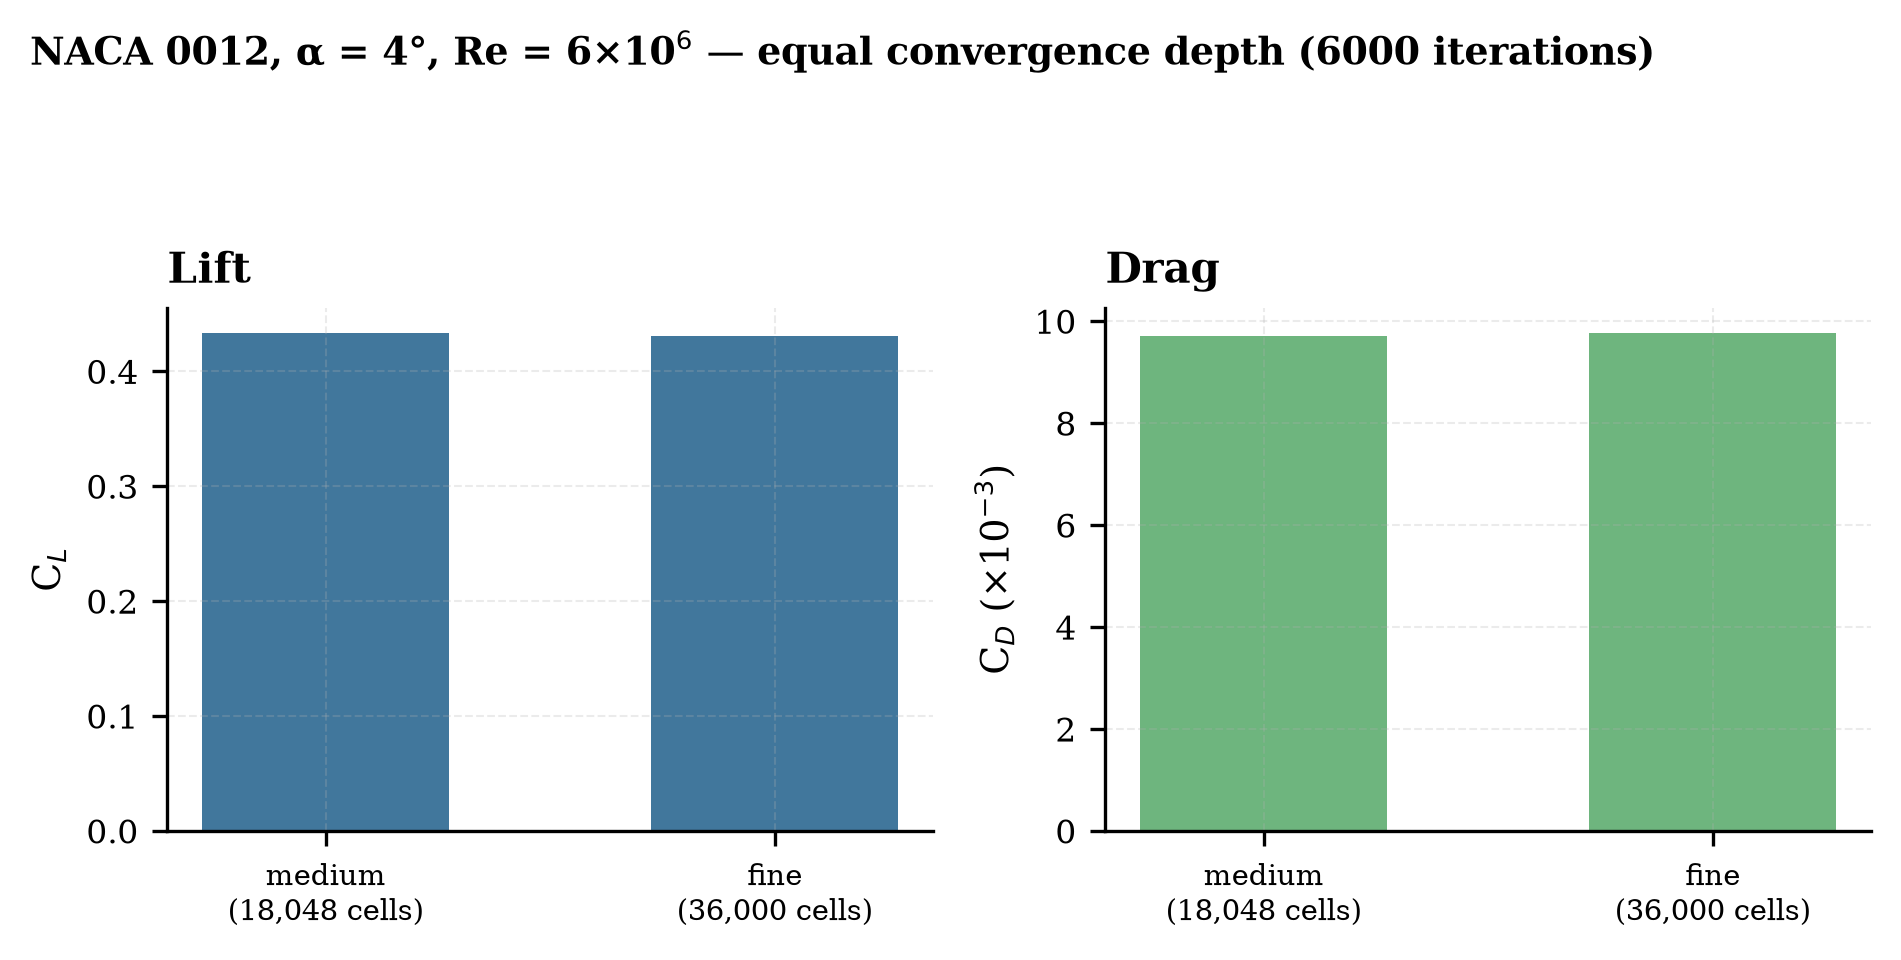
\includegraphics[width=0.85\textwidth]{figures/fig_mesh.png}
\caption{Grid sensitivity at equal convergence depth (6000 iterations,
converged). Medium and fine meshes agree closely; coarse inflates drag.}
\label{fig:mesh}
\end{figure}

\subsection{Physical consistency of the dataset}

Per-airfoil lift slopes fitted over $|\alpha| \le 6^\circ$ span
5.16--6.24~rad$^{-1}$ with median 5.89, i.e.\ $\approx 94\%$ of thin-airfoil
theory, and rise systematically with Reynolds number
(Figure~\ref{fig:slope})---the expected signature of shrinking viscous
displacement effects. No converged row contains negative drag, non-finite
coefficients or $|C_L|$ beyond 2.2.

\begin{figure}[htbp]
\centering
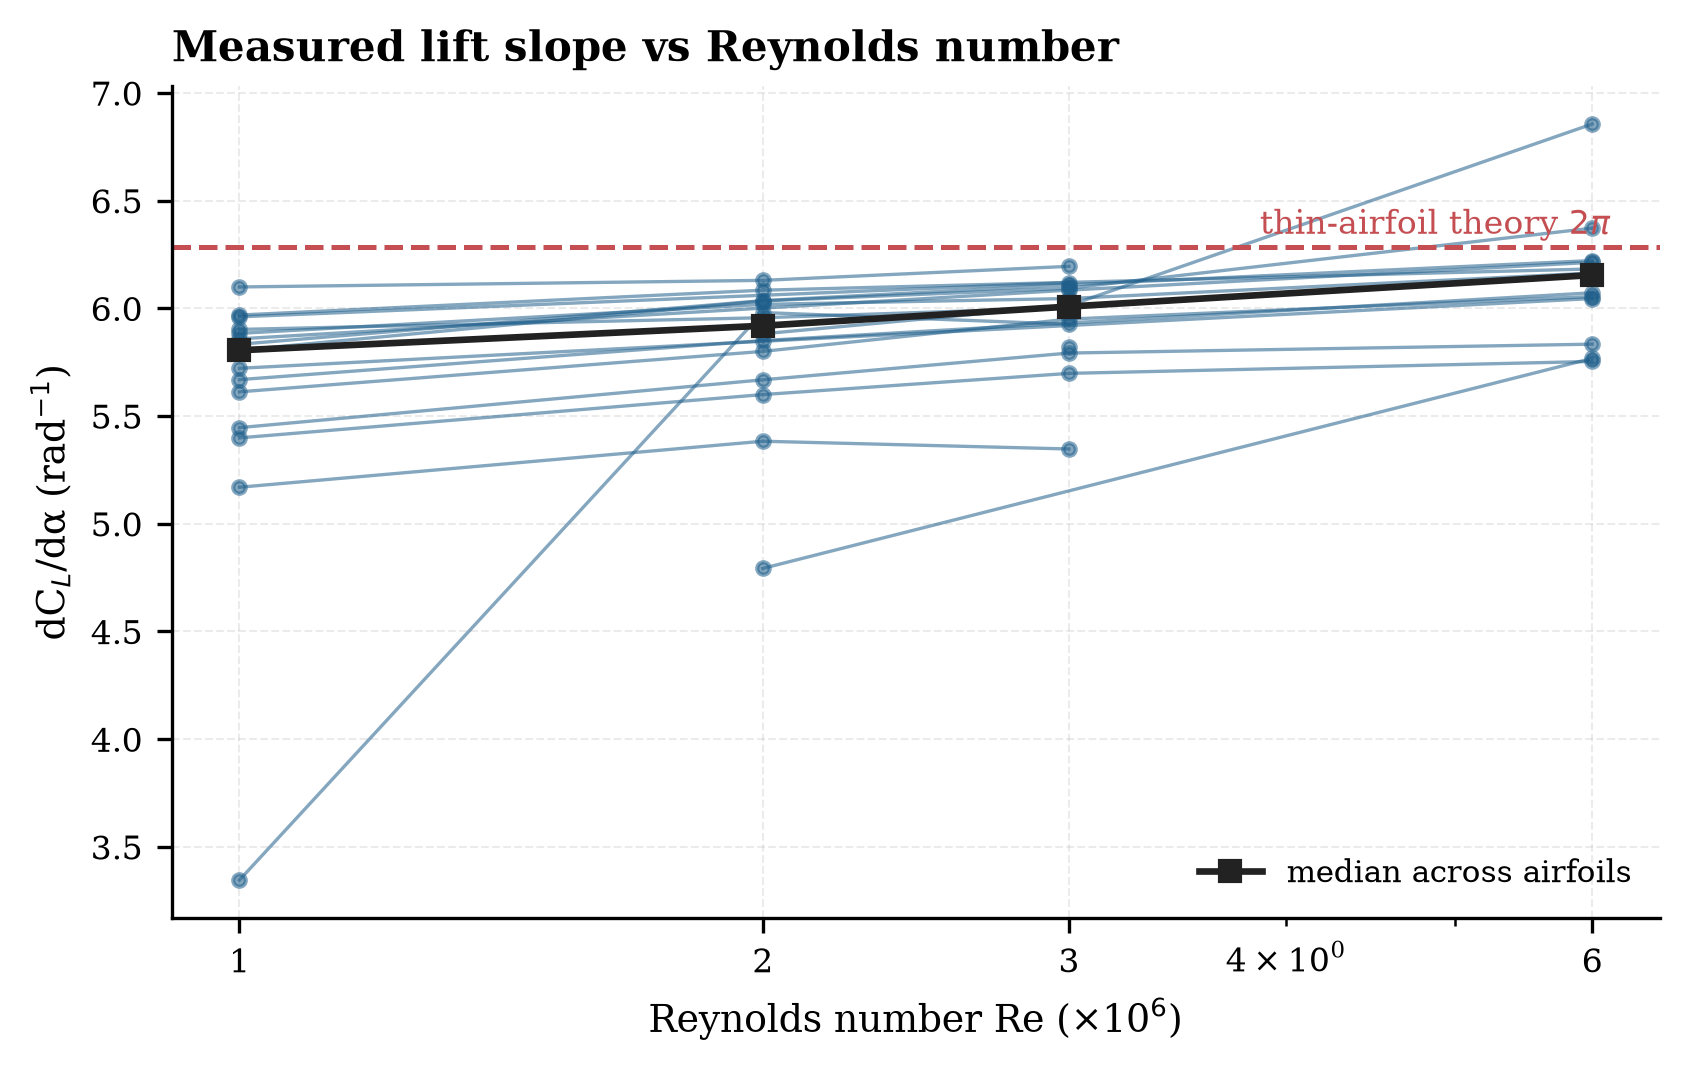
\includegraphics[width=0.85\textwidth]{figures/fig_lift_slope.png}
\caption{Lift slope against Reynolds number for every airfoil with at least
three converged points in the attached range; dashed line: thin-airfoil
theory $2\pi$.}
\label{fig:slope}
\end{figure}

\section{Dataset statistics and the exclusion study}

\subsection{Coverage}

\begin{table}[htbp]
\centering
\caption{Final campaign composition (504-case production grid).}
\label{tab:composition}
\begin{tabular}{lrl}
\toprule
Outcome & Cases & Meaning \\
\midrule
Converged & 374 & strict criteria met; training-eligible \\
Unconverged & 26 & solved and extracted; excluded from training \\
Solver crashed / timed out & 10 & diverged (SIGFPE) or hit the time cap \\
Never attempted & 94 & deferred after the third failure wave \\
\midrule
Production coverage & \textbf{400/504} & \\
\bottomrule
\end{tabular}
\end{table}

All 21 airfoils retain converged rows at all four Reynolds numbers
(8--24 rows each). The 31 empty cells of the airfoil--$\alpha$ coverage map
(Figure~\ref{fig:coverage}) concentrate on thin airfoils at stall and
negative incidence---precisely the regimes the exclusion study identifies as
unsteady. At inference these regimes are covered by the domain-applicability
guard rather than by extrapolated training data.

\begin{figure}[htbp]
\centering
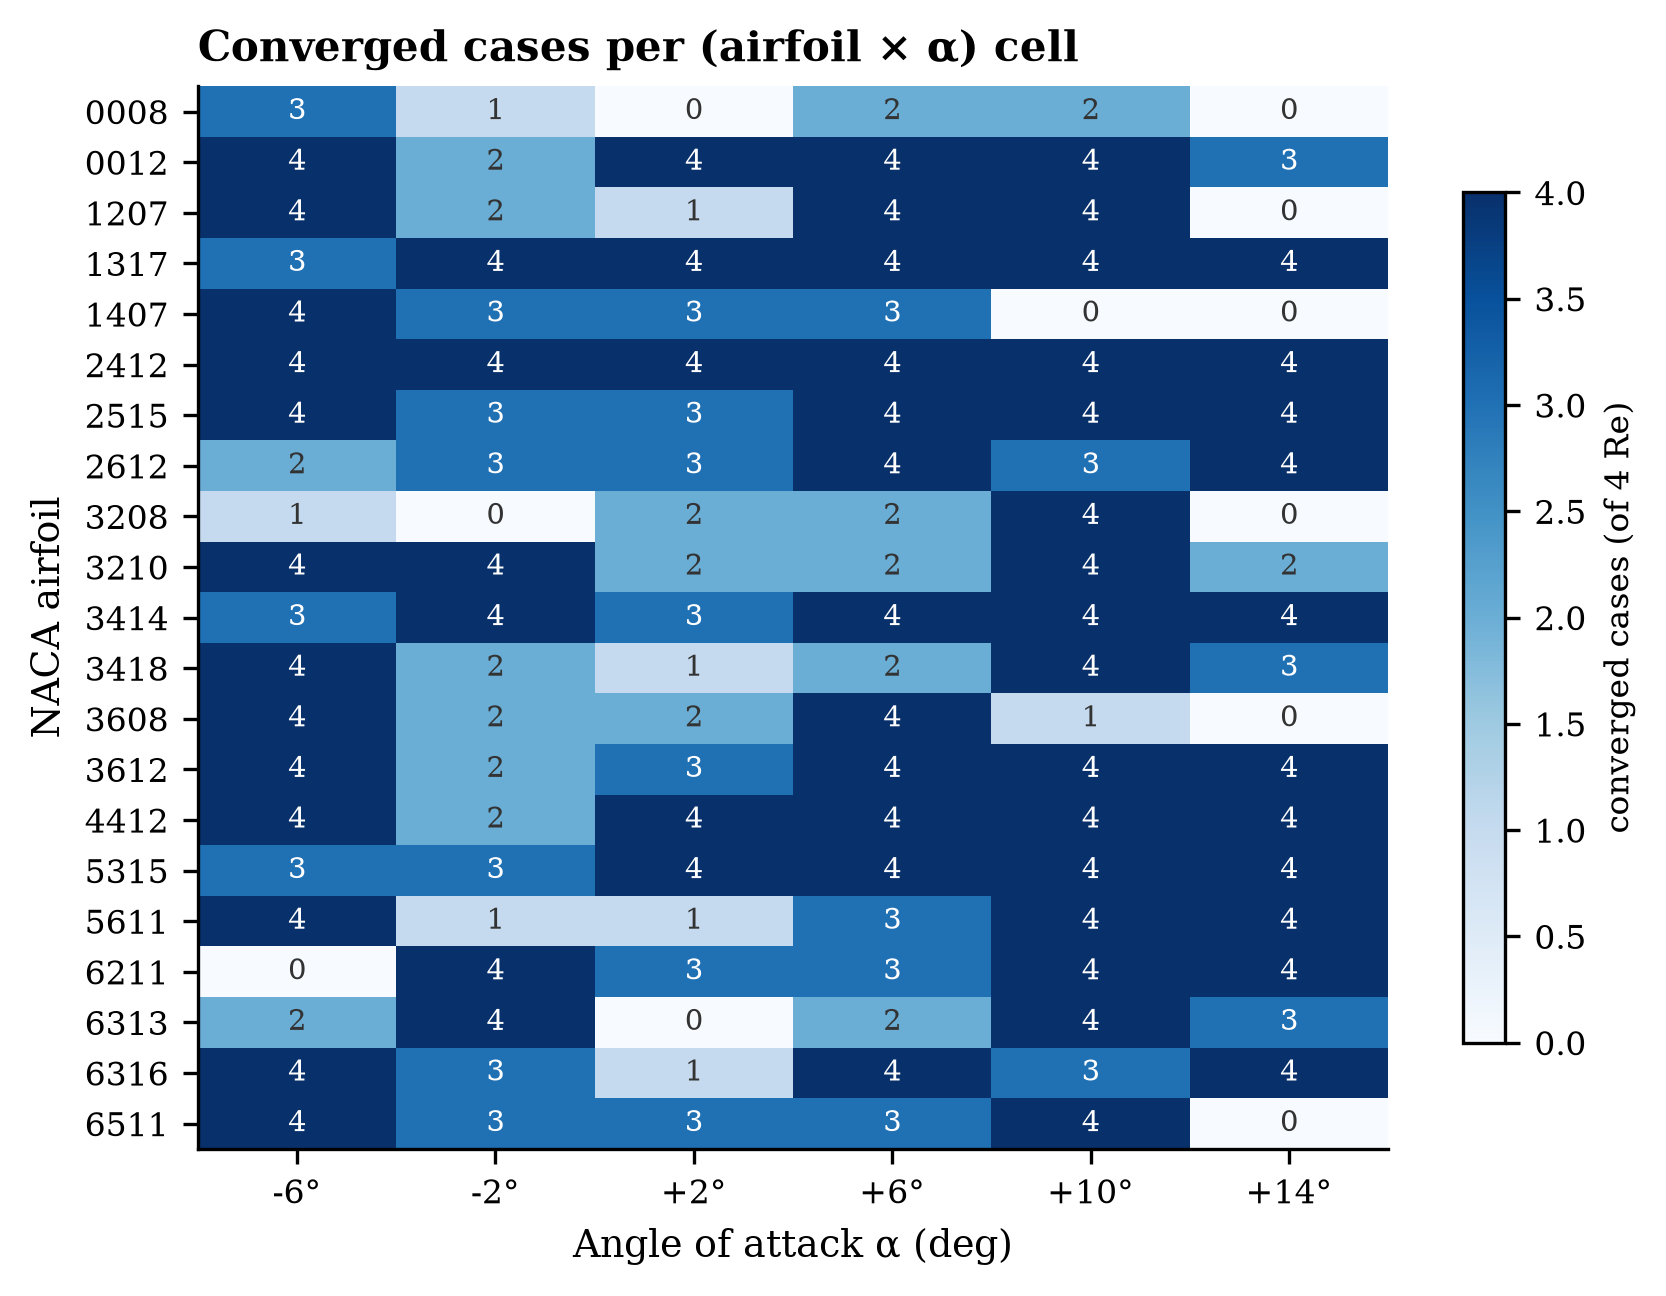
\includegraphics[width=0.78\textwidth]{figures/fig_coverage.png}
\caption{Converged cases per (airfoil $\times$ $\alpha$) cell. Empty cells are
the physically unsteady population, not random gaps.}
\label{fig:coverage}
\end{figure}

\subsection{Campaign effort}

Wall times ranged from $\approx 180$~s (3000-iteration pass, one core) to
$\approx 590$--$730$~s (6000-iteration budget under six-way concurrency), with
mesh failures rejected in $\approx 1$~s and divergent crashes at 150--420~s
(Figure~\ref{fig:walltime}). The full campaign plus recovery passes represents
roughly 80 core-hours of OpenFOAM execution on consumer and university
hardware, fully checkpointed.

\begin{figure}[htbp]
\centering
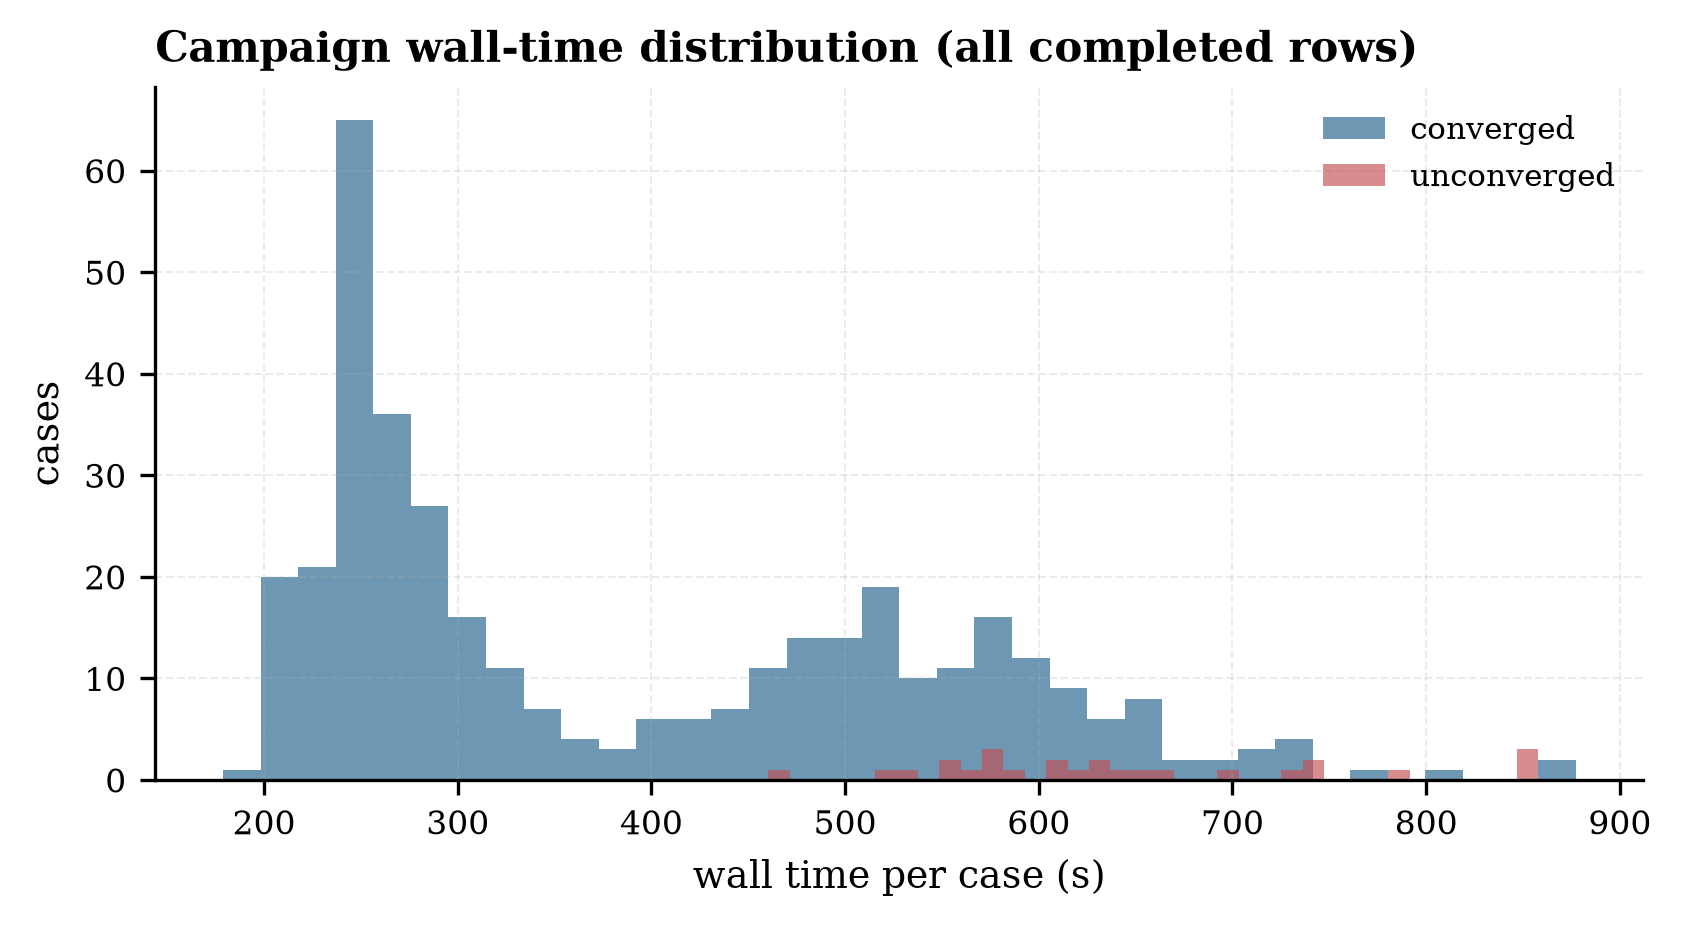
\includegraphics[width=0.85\textwidth]{figures/fig_walltime.png}
\caption{Wall-time distribution of completed cases.}
\label{fig:walltime}
\end{figure}

\subsection{Why 104 cases are excluded: limit cycles, not defects}

The excluded cases share a measurable signature. Their $C_L$ histories
oscillate with peak-to-peak amplitudes 10--50$\times$ the convergence
tolerance while the mean drifts slowly; the variability spectrum is continuous
across the criterion boundary (converged 95th percentile
$4.5\times10^{-4}$ versus unconverged minimum $5.9\times10^{-4}$), so the
criterion draws a line through a smooth population rather than separating two
distinct ones
(Figure~\ref{fig:limitcycle}). Physically these are mildly separated,
negative-incidence and near-stall flows for which the steady RANS equations
admit no stable fixed point: the residual field settles into a slow limit
cycle that no iteration budget at these settings removes. Three independent
attempts (3000 iterations, 6000 iterations, and 6000 with a doubled time cap)
reproduced the same outcomes, confirming the cause is physical rather than
procedural. Training on such rows would inject oscillating, mean-drifting
targets with no steady truth to learn; exclusion is the honest treatment, and
a hybrid steady/unsteady driver that returns time-averaged means with an
unsteadiness band is the identified v2 remedy.

\begin{figure}[htbp]
\centering
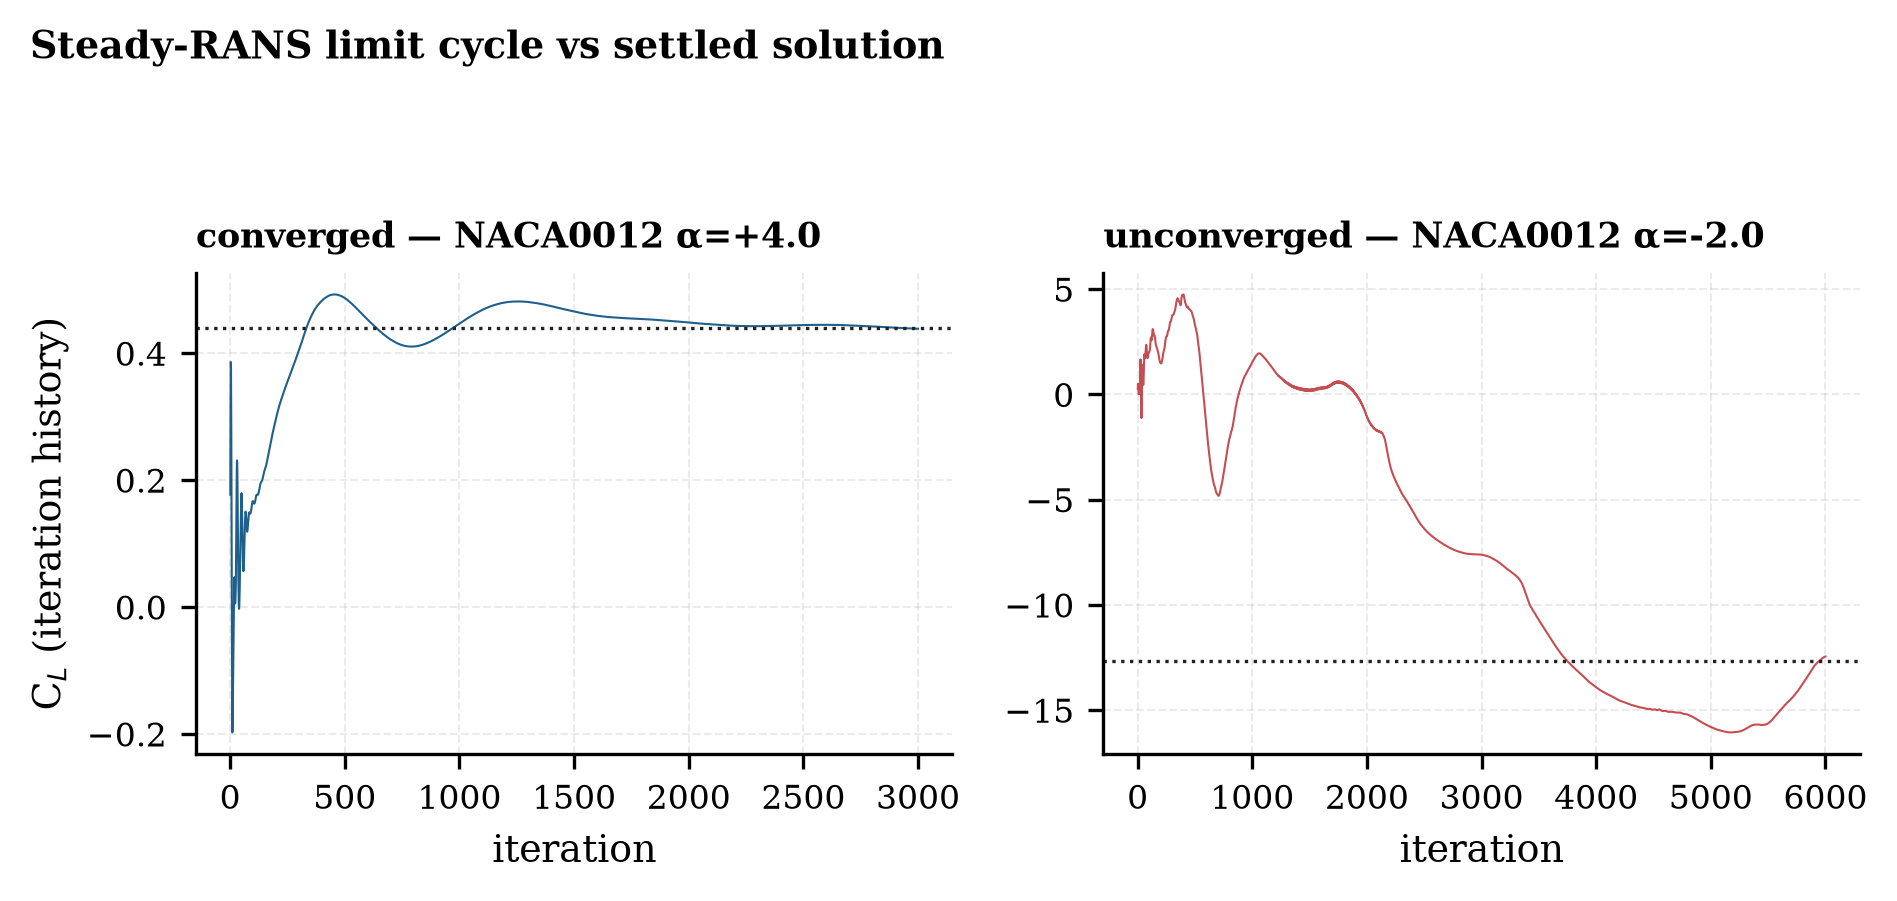
\includegraphics[width=0.98\textwidth]{figures/fig_limit_cycle.png}
\caption{Force-coefficient histories. Left: a converged case settles to a
flat line. Right: an excluded case oscillates around a drifting mean---the
steady solver has no fixed point at this operating point.}
\label{fig:limitcycle}
\end{figure}

\section{Surrogate models}

\subsection{Architecture and training}

The scalar head is a deep residual MLP (batch-normalised input and residual
blocks, GELU activations) mapping 17 features---m, p, t, six upper and six
lower CST coefficients, $\alpha$ and $Re$---to $C_L$, $C_D$, $C_m$. The field
head is a physics-informed decoder that emits 322 pressure values (161 upper
and 161 lower chord stations) per operating point. Both are trained on the
375 converged rows with a grouped split: entire airfoils are held out for
testing (NACA 3414, 5315, 5611), so every test point is an extrapolation to
an unseen geometry. Training ran on an NVIDIA GPU (Kaggle) with deterministic
seeding; the exported bundle contains pure-NumPy weights, scalers and
conformal quantiles so inference needs no deep-learning runtime. A
\emph{leakage diagnostic} reports both splits side by side rather than the
favourable one alone (Table~\ref{tab:r2}).

\subsection{Grouped-holdout results}

\begin{table}[htbp]
\centering
\caption{Scalar test metrics: grouped per-airfoil holdout (extrapolation to
unseen airfoils) versus random-row split (interpolation). Test airfoils:
NACA 3414, 5315, 5611.}
\label{tab:r2}
\small
\setlength{\tabcolsep}{4.5pt}
\begin{tabular}{lccc|ccc}
\toprule
& \multicolumn{3}{c|}{Grouped (unseen)} & \multicolumn{3}{c}{Random (interp.)} \\
Target & $R^2$ & RMSE & MAE & $R^2$ & RMSE & MAE \\
\midrule
$C_L$ & 0.966 & 0.1147 & 0.0953 & 0.9954 & 0.0477 & 0.0387 \\
$C_D$ & 0.933 & 0.00368 & 0.00218 & 0.9743 & 0.00123 & 0.00088 \\
$C_m$ & 0.860 & 0.01668 & 0.01140 & 0.9956 & 0.00300 & 0.00240 \\
\bottomrule
\end{tabular}
\end{table}

The interpolation--extrapolation gap ($C_L$ 0.995$\to$0.966, $C_D$
0.974$\to$0.933, $C_m$ 0.996$\to$0.860) is reported as the honest
generalisation cost of geometry transfer.

\subsection{Surface pressure and physics consistency}

The Cp decoder reaches $R^2 = 0.892$ (RMSE 0.326) on the held-out airfoils.
Because lift is the chordwise integral of the pressure difference, the
decoder's output can be checked against the scalar head:
integrating the predicted $\Delta C_p$ reproduces the predicted $C_L$ with
$R^2 = 0.983$---the two heads are consistent with each other and with the
flow physics. Figure~\ref{fig:cp} compares measured and predicted surface
pressure on held-out geometries.

\begin{figure}[htbp]
\centering
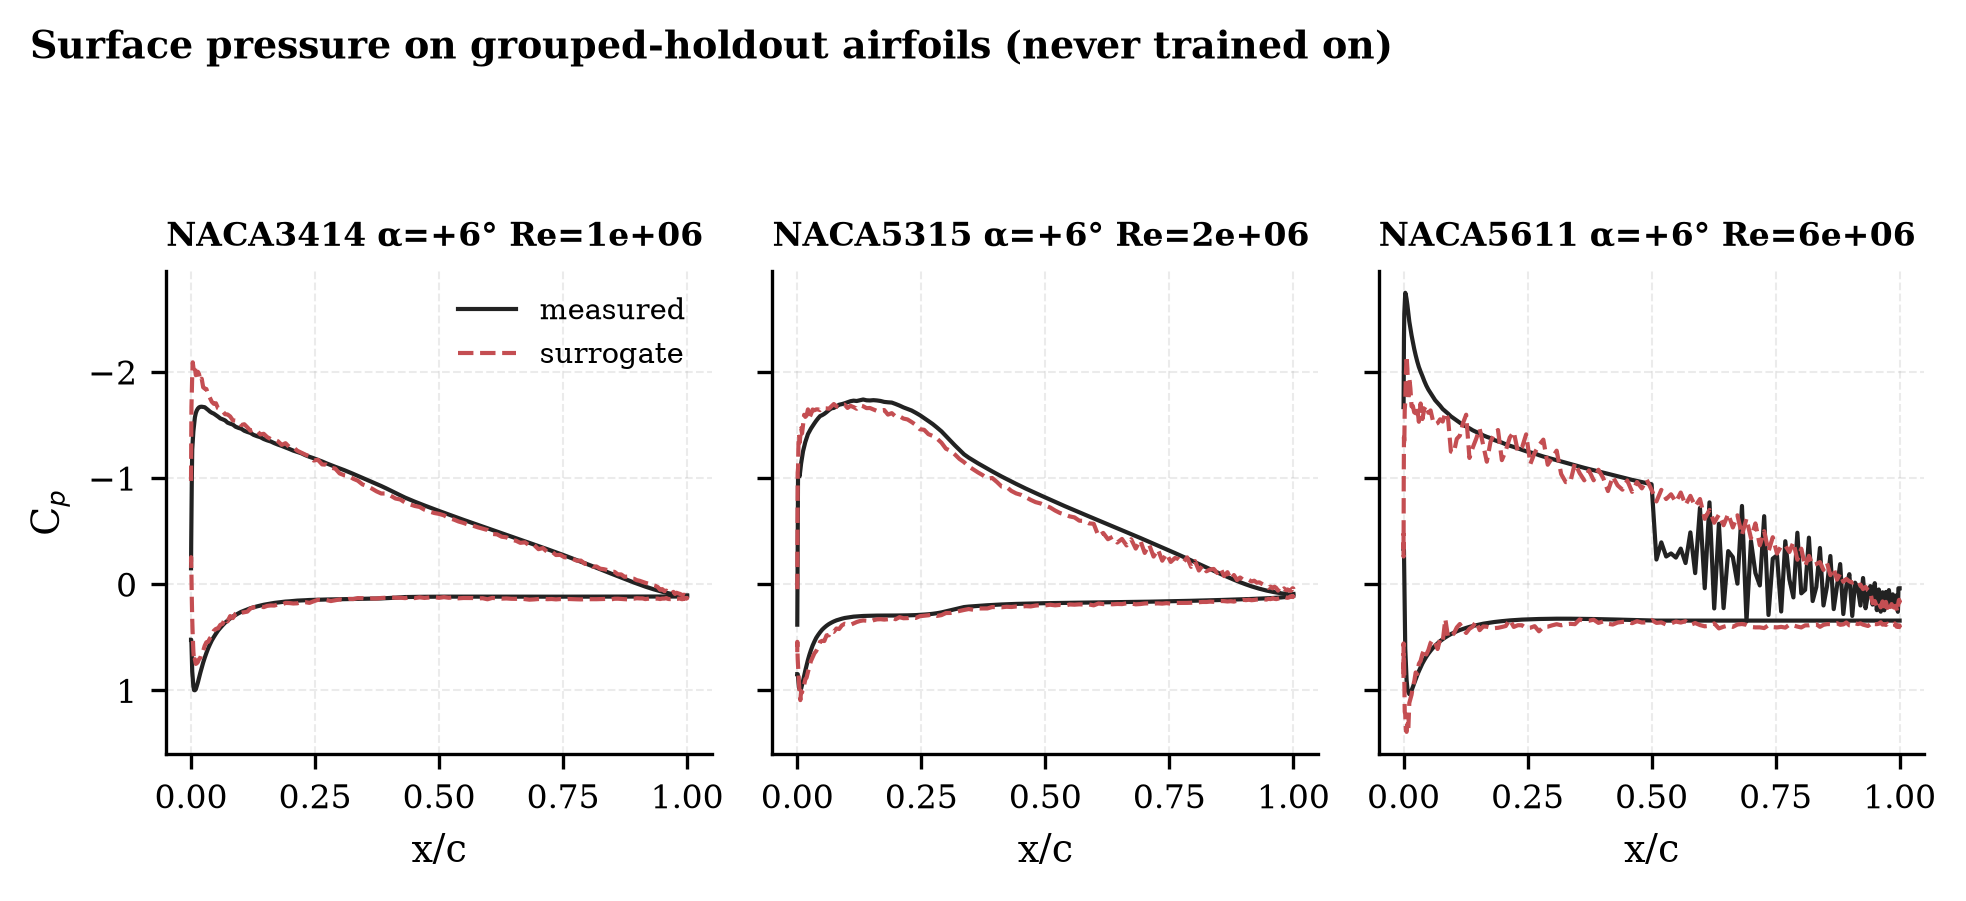
\includegraphics[width=0.98\textwidth]{figures/fig_cp_holdout.png}
\caption{Measured (solid) versus surrogate-predicted (dashed) surface
pressure on grouped-holdout airfoils never seen in training.}
\label{fig:cp}
\end{figure}

\begin{figure}[htbp]
\centering
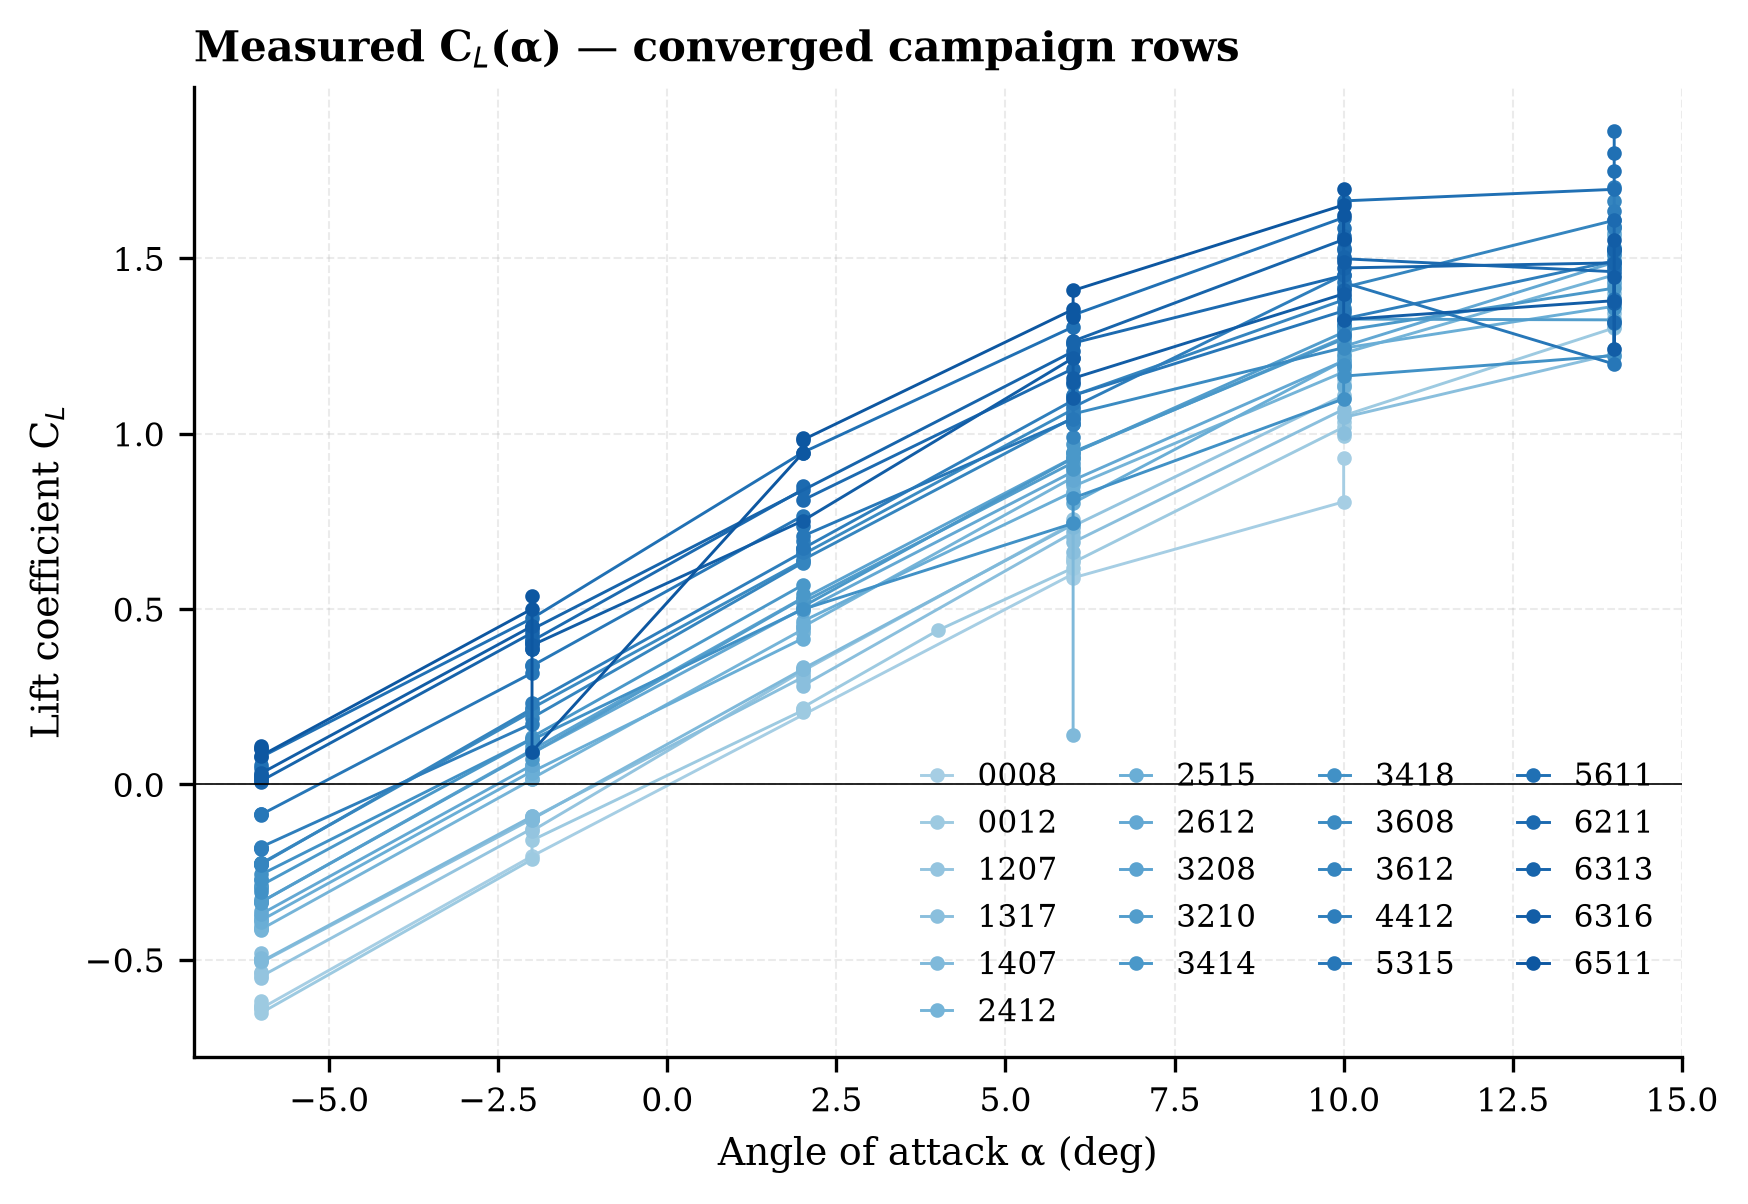
\includegraphics[width=0.85\textwidth]{figures/fig_cl_alpha.png}
\caption{Measured $C_L(\alpha)$ across the 21-airfoil family (converged
rows).}
\label{fig:clalpha}
\end{figure}

\subsection{Conformal calibration and empirical coverage}

Split-conformal quantiles of held-out absolute residuals ($q_{C_L}=0.229$,
$q_{C_D}=0.00695$, $q_{C_m}=0.0390$, plus per-chord-station $C_p$ quantiles)
are exported with the bundle from a 52-row calibration set. On the
unseen-airfoil test set the empirical coverage is:

\begin{table}[htbp]
\centering
\caption{Empirical conformal coverage on unseen airfoils versus the 0.95
nominal level.}
\label{tab:coverage}
\begin{tabular}{lcc}
\toprule
Quantity & Empirical coverage & Nominal \\
\midrule
$C_L$ & 0.951 & 0.95 \\
$C_D$ & 0.918 & 0.95 \\
$C_m$ & 0.967 & 0.95 \\
$C_p$ (combined) & 0.957 & 0.95 \\
\bottomrule
\end{tabular}
\end{table}

\subsection{Domain applicability}

A Mahalanobis distance over the (m, p, t, $\alpha$, $Re$) feature space
separates in-domain from out-of-domain queries: seen-airfoil rows have median
distance 3.56 (99th percentile 4.45), while held-out-airfoil rows reach a
median of 6.60 and a maximum of 18.8, with 63.9\% beyond the
$\chi^2(0.99)$ threshold. Queries outside the calibrated domain are labelled
as such and served with widened analytic bands instead of conformal
intervals---the engine never presents an extrapolation as an interpolation.

\section{Limitations}

\begin{itemize}
\item \textbf{Regime.} Two-dimensional, incompressible, fully turbulent RANS
($k$--$\omega$ SST, no transition model) over the NACA four-digit family at
$10^6$--$6\times10^6$ Reynolds. The surrogate is valid inside that envelope
and flagged outside it; drag is biased high relative to transitional
experimental data by the absence of a transition model.
\item \textbf{Coverage.} 104 of 504 operating points are excluded. They are a
physically coherent population (negative-$\alpha$/stall limit cycles), but
the surrogate interpolates cautiously there via other shapes rather than
learning them directly.
\item \textbf{Convergence depth.} The 3000-iteration production rows carry a
quantified $\approx 1.3\%$ ($C_L$) and $\approx 2.4\%$ ($C_D$) systematic
offset relative to deeper convergence; the recovery pass used 6000 iterations.
\item \textbf{Calibration size.} The conformal calibration set is 52 rows;
coverage is honest but the quantiles are estimated from a modest sample.
\item \textbf{Geometry family.} CST weights enable smooth interpolation within
the sampled manifold, but shapes far outside it are extrapolations and will
be flagged as such.
\end{itemize}

\section{Outlook}

The identified v2 remedy for the excluded population is a hybrid
steady/unsteady driver: run steady SIMPLE, detect the limit cycle with the
same window criterion, switch automatically to a PIMPLE unsteady phase, and
return time-averaged coefficients with an unsteadiness band. That converts
the excluded operating points into a new, honestly-labelled data tier and
would take the dataset to full-grid coverage. A second direction is
deploying a tensor-basis neural-network closure (tbnnFoam) on the same cases
to test whether a learned anisotropy model stabilises steady solutions that
linear eddy-viscosity closures cannot. The Streamlit interface is planned
after the dataset and models, presenting every query with its backend,
provenance, conformal band and domain-applicability status.

\section{Reproducibility}

The repository contains the complete chain: campaign driver with adaptive
mesh fallback, iteration override and checkpoint pruning
(\path{scripts/run_dataset_campaign.py},
\path{scripts/prune_checkpoint_rows.py});
quality-control audit (\path{scripts/qc_campaign.py}, reports under
\path{reports/qc/}); mesh-sensitivity study
(\path{scripts/run_mesh_sensitivity.py}, \path{reports/mesh_study/});
the training notebook builder and its contract tests
(\path{scripts/build_kaggle_notebook_v2.py},
\path{tests/test_training_notebook_contract.py});
and the inference engine with its backend, provenance and UQ tests
(\path{src/models/inference.py},
\path{tests/test_inference_backend.py}). The shipped bundle loads with:

\begin{quote}
\texttt{engine = AeroSurrogateEngine()}\\
\texttt{result = engine.predict(}\\
\texttt{\hphantom{result = engine.}m=0.02, p=0.4, t=0.12, alpha\_deg=4.0)}
\end{quote}

returning coefficients, the full surface-pressure field, conformal intervals
and the domain-applicability report for every query.

\begin{table}[htbp]
\centering
\caption{Primary repository artifacts and their locations.}
\label{tab:artifacts}
\begin{tabular}{ll}
\toprule
Artifact & Location \\
\midrule
Real-CFD dataset (CSV + Cp fields) & \texttt{data/processed/} \\
Trained model bundle (\texttt{openfoam} provenance) & \texttt{models/} \\
Legacy synthetic artifacts (archived) & \texttt{models/legacy\_synthetic/} \\
\phantom{Legacy synthetic artifacts (archived)} & \texttt{data/processed/legacy\_synthetic/} \\
Quality-control audit & \texttt{reports/qc/} \\
Mesh-sensitivity study & \texttt{reports/mesh\_study/} \\
Campaign logs (resume checkpoint trail) & \texttt{data/raw\_cases/}, \texttt{campaign\_*.log} \\
Snapshot copies & \texttt{data/snapshots/} \\
Training notebook builder + contract tests & \texttt{scripts/build\_kaggle\_notebook\_v2.py} \\
\bottomrule
\end{tabular}
\end{table}

\end{document}
